% Options for packages loaded elsewhere
\PassOptionsToPackage{unicode}{hyperref}
\PassOptionsToPackage{hyphens}{url}
%
\documentclass[
]{book}
\usepackage{amsmath,amssymb}
\usepackage{lmodern}
\usepackage{iftex}
\ifPDFTeX
  \usepackage[T1]{fontenc}
  \usepackage[utf8]{inputenc}
  \usepackage{textcomp} % provide euro and other symbols
\else % if luatex or xetex
  \usepackage{unicode-math}
  \defaultfontfeatures{Scale=MatchLowercase}
  \defaultfontfeatures[\rmfamily]{Ligatures=TeX,Scale=1}
\fi
% Use upquote if available, for straight quotes in verbatim environments
\IfFileExists{upquote.sty}{\usepackage{upquote}}{}
\IfFileExists{microtype.sty}{% use microtype if available
  \usepackage[]{microtype}
  \UseMicrotypeSet[protrusion]{basicmath} % disable protrusion for tt fonts
}{}
\makeatletter
\@ifundefined{KOMAClassName}{% if non-KOMA class
  \IfFileExists{parskip.sty}{%
    \usepackage{parskip}
  }{% else
    \setlength{\parindent}{0pt}
    \setlength{\parskip}{6pt plus 2pt minus 1pt}}
}{% if KOMA class
  \KOMAoptions{parskip=half}}
\makeatother
\usepackage{xcolor}
\IfFileExists{xurl.sty}{\usepackage{xurl}}{} % add URL line breaks if available
\IfFileExists{bookmark.sty}{\usepackage{bookmark}}{\usepackage{hyperref}}
\hypersetup{
  pdftitle={Course Outline: Time Series Data in R},
  pdfauthor={Harrison Brown},
  hidelinks,
  pdfcreator={LaTeX via pandoc}}
\urlstyle{same} % disable monospaced font for URLs
\usepackage{color}
\usepackage{fancyvrb}
\newcommand{\VerbBar}{|}
\newcommand{\VERB}{\Verb[commandchars=\\\{\}]}
\DefineVerbatimEnvironment{Highlighting}{Verbatim}{commandchars=\\\{\}}
% Add ',fontsize=\small' for more characters per line
\usepackage{framed}
\definecolor{shadecolor}{RGB}{248,248,248}
\newenvironment{Shaded}{\begin{snugshade}}{\end{snugshade}}
\newcommand{\AlertTok}[1]{\textcolor[rgb]{0.94,0.16,0.16}{#1}}
\newcommand{\AnnotationTok}[1]{\textcolor[rgb]{0.56,0.35,0.01}{\textbf{\textit{#1}}}}
\newcommand{\AttributeTok}[1]{\textcolor[rgb]{0.77,0.63,0.00}{#1}}
\newcommand{\BaseNTok}[1]{\textcolor[rgb]{0.00,0.00,0.81}{#1}}
\newcommand{\BuiltInTok}[1]{#1}
\newcommand{\CharTok}[1]{\textcolor[rgb]{0.31,0.60,0.02}{#1}}
\newcommand{\CommentTok}[1]{\textcolor[rgb]{0.56,0.35,0.01}{\textit{#1}}}
\newcommand{\CommentVarTok}[1]{\textcolor[rgb]{0.56,0.35,0.01}{\textbf{\textit{#1}}}}
\newcommand{\ConstantTok}[1]{\textcolor[rgb]{0.00,0.00,0.00}{#1}}
\newcommand{\ControlFlowTok}[1]{\textcolor[rgb]{0.13,0.29,0.53}{\textbf{#1}}}
\newcommand{\DataTypeTok}[1]{\textcolor[rgb]{0.13,0.29,0.53}{#1}}
\newcommand{\DecValTok}[1]{\textcolor[rgb]{0.00,0.00,0.81}{#1}}
\newcommand{\DocumentationTok}[1]{\textcolor[rgb]{0.56,0.35,0.01}{\textbf{\textit{#1}}}}
\newcommand{\ErrorTok}[1]{\textcolor[rgb]{0.64,0.00,0.00}{\textbf{#1}}}
\newcommand{\ExtensionTok}[1]{#1}
\newcommand{\FloatTok}[1]{\textcolor[rgb]{0.00,0.00,0.81}{#1}}
\newcommand{\FunctionTok}[1]{\textcolor[rgb]{0.00,0.00,0.00}{#1}}
\newcommand{\ImportTok}[1]{#1}
\newcommand{\InformationTok}[1]{\textcolor[rgb]{0.56,0.35,0.01}{\textbf{\textit{#1}}}}
\newcommand{\KeywordTok}[1]{\textcolor[rgb]{0.13,0.29,0.53}{\textbf{#1}}}
\newcommand{\NormalTok}[1]{#1}
\newcommand{\OperatorTok}[1]{\textcolor[rgb]{0.81,0.36,0.00}{\textbf{#1}}}
\newcommand{\OtherTok}[1]{\textcolor[rgb]{0.56,0.35,0.01}{#1}}
\newcommand{\PreprocessorTok}[1]{\textcolor[rgb]{0.56,0.35,0.01}{\textit{#1}}}
\newcommand{\RegionMarkerTok}[1]{#1}
\newcommand{\SpecialCharTok}[1]{\textcolor[rgb]{0.00,0.00,0.00}{#1}}
\newcommand{\SpecialStringTok}[1]{\textcolor[rgb]{0.31,0.60,0.02}{#1}}
\newcommand{\StringTok}[1]{\textcolor[rgb]{0.31,0.60,0.02}{#1}}
\newcommand{\VariableTok}[1]{\textcolor[rgb]{0.00,0.00,0.00}{#1}}
\newcommand{\VerbatimStringTok}[1]{\textcolor[rgb]{0.31,0.60,0.02}{#1}}
\newcommand{\WarningTok}[1]{\textcolor[rgb]{0.56,0.35,0.01}{\textbf{\textit{#1}}}}
\usepackage{longtable,booktabs,array}
\usepackage{calc} % for calculating minipage widths
% Correct order of tables after \paragraph or \subparagraph
\usepackage{etoolbox}
\makeatletter
\patchcmd\longtable{\par}{\if@noskipsec\mbox{}\fi\par}{}{}
\makeatother
% Allow footnotes in longtable head/foot
\IfFileExists{footnotehyper.sty}{\usepackage{footnotehyper}}{\usepackage{footnote}}
\makesavenoteenv{longtable}
\usepackage{graphicx}
\makeatletter
\def\maxwidth{\ifdim\Gin@nat@width>\linewidth\linewidth\else\Gin@nat@width\fi}
\def\maxheight{\ifdim\Gin@nat@height>\textheight\textheight\else\Gin@nat@height\fi}
\makeatother
% Scale images if necessary, so that they will not overflow the page
% margins by default, and it is still possible to overwrite the defaults
% using explicit options in \includegraphics[width, height, ...]{}
\setkeys{Gin}{width=\maxwidth,height=\maxheight,keepaspectratio}
% Set default figure placement to htbp
\makeatletter
\def\fps@figure{htbp}
\makeatother
\setlength{\emergencystretch}{3em} % prevent overfull lines
\providecommand{\tightlist}{%
  \setlength{\itemsep}{0pt}\setlength{\parskip}{0pt}}
\setcounter{secnumdepth}{5}
\usepackage{booktabs}
\ifLuaTeX
  \usepackage{selnolig}  % disable illegal ligatures
\fi
\usepackage[]{natbib}
\bibliographystyle{plainnat}

\title{Course Outline: Time Series Data in R}
\author{Harrison Brown}
\date{2022-05-04}

\begin{document}
\maketitle

{
\setcounter{tocdepth}{1}
\tableofcontents
}
\hypertarget{welcome}{%
\chapter*{Welcome}\label{welcome}}
\addcontentsline{toc}{chapter}{Welcome}

Welcome to the course outline for \emph{Time Series Data in R}! This course offers methods and workflows for analyzing and interpreting time series data, an overview of when, why, and how to use time series data, and various utilities and packages in R that are beneficial to analysts.

By the end of this course, students will have the skills to:

\begin{itemize}
\tightlist
\item
  Interpret and understand time series plots
\item
  Import ts data to create and manipulate \texttt{ts} objects from the \texttt{stats} package
\item
  Understand why time series data is fundamentally different than non-ts data.
\item
  Analyze time series data with plots
\item
  ?Intro to Wavelet analysis?
\end{itemize}

\hypertarget{introduction-to-time-series-data}{%
\chapter{Introduction to time series data}\label{introduction-to-time-series-data}}

\hypertarget{what-is-a-time-series}{%
\section{What is a time series}\label{what-is-a-time-series}}

\begin{itemize}
\tightlist
\item
  Sampled at equi-spaced points in time
\end{itemize}

\hypertarget{stationary-vs-non-stationary-series}{%
\section{Stationary vs Non-Stationary series}\label{stationary-vs-non-stationary-series}}

Non-stationary time series are defined by:

\begin{itemize}
\tightlist
\item
  Time-dependent Mean
\item
  Time-dependent Variance
\item
  Time-dependent Autocorrelation/Covariance
\end{itemize}

\hypertarget{dickey-fuller-test-of-stationarity}{%
\section{Dickey-Fuller Test of Stationarity}\label{dickey-fuller-test-of-stationarity}}

\hypertarget{creating-and-manipulating-time-series}{%
\chapter{Creating and Manipulating Time Series}\label{creating-and-manipulating-time-series}}

\hypertarget{ts-class}{%
\section{\texorpdfstring{\texttt{ts} Class}{ts Class}}\label{ts-class}}

\hypertarget{creating-a-ts.plot}{%
\section{\texorpdfstring{Creating a \texttt{ts.plot()}}{Creating a ts.plot()}}\label{creating-a-ts.plot}}

\hypertarget{interpreting-plots}{%
\subsection{Interpreting Plots}\label{interpreting-plots}}

\hypertarget{seasonality-plot}{%
\subsection{Seasonality Plot}\label{seasonality-plot}}

\begin{Shaded}
\begin{Highlighting}[]
\FunctionTok{ggseasonplot}\NormalTok{(}\AttributeTok{x =}\NormalTok{ AirPassengers)}
\end{Highlighting}
\end{Shaded}

\begin{center}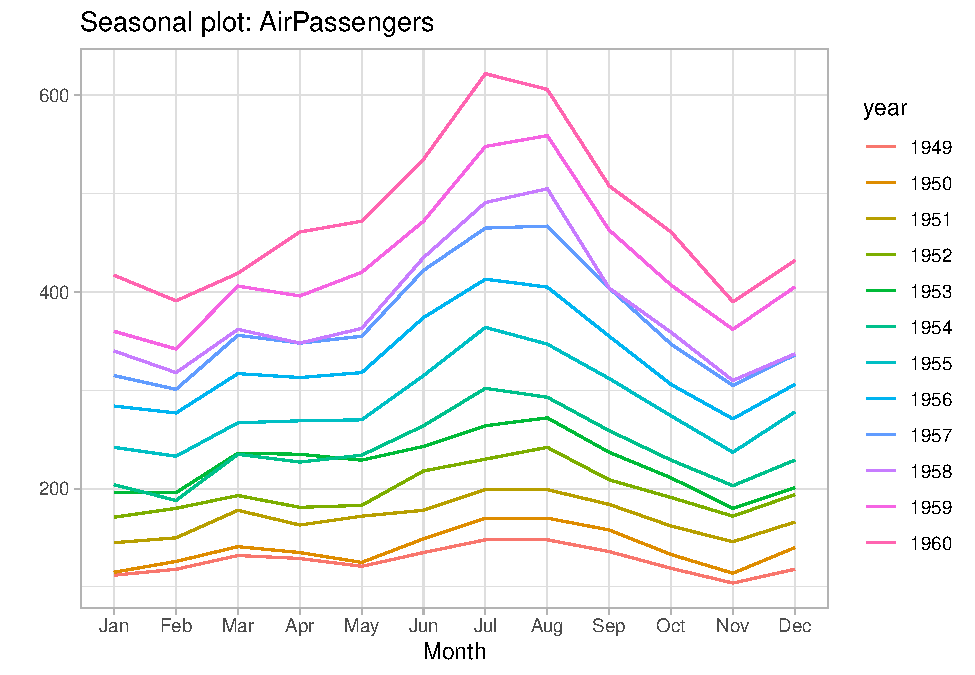
\includegraphics{_main_files/figure-latex/season-1-1} \end{center}

\hypertarget{polar-seasonality-plot}{%
\subsection{Polar Seasonality Plot}\label{polar-seasonality-plot}}

\hypertarget{trends-and-seasons}{%
\section{Trends and Seasons}\label{trends-and-seasons}}

\hypertarget{decomposition}{%
\subsection{Decomposition}\label{decomposition}}

\hypertarget{de-trending-data}{%
\subsection{De-trending Data}\label{de-trending-data}}

\hypertarget{rolling-and-expanding-windows}{%
\chapter{Rolling and Expanding Windows}\label{rolling-and-expanding-windows}}

\hypertarget{rolling-window}{%
\section{Rolling Window}\label{rolling-window}}

\begin{itemize}
\tightlist
\item
  Moving lower and upper bound
\end{itemize}

\hypertarget{data}{%
\subsection{Data}\label{data}}

\begin{Shaded}
\begin{Highlighting}[]
\FunctionTok{library}\NormalTok{(tsbox)}

\NormalTok{dl\_dplyr }\OtherTok{\textless{}{-}}\NormalTok{ cran\_data }\SpecialCharTok{\%\textgreater{}\%}
  \FunctionTok{filter}\NormalTok{(date }\SpecialCharTok{\textgreater{}=} \FunctionTok{as.Date}\NormalTok{(}\StringTok{"2018{-}01{-}01"}\NormalTok{)) }\SpecialCharTok{\%\textgreater{}\%} 
  \FunctionTok{select}\NormalTok{(}\SpecialCharTok{{-}}\NormalTok{package)}

\CommentTok{\# tsbox::ts\_ts() parses the Date column in a much easier way, making the}
\CommentTok{\# conversion process easy to interpret}
\NormalTok{dl\_ts }\OtherTok{\textless{}{-}}\NormalTok{ dl\_dplyr }\SpecialCharTok{\%\textgreater{}\%}
\NormalTok{  tsbox}\SpecialCharTok{::}\FunctionTok{ts\_ts}\NormalTok{()}
\end{Highlighting}
\end{Shaded}

\begin{verbatim}
## [time]: 'date' [value]: 'count'
\end{verbatim}

\begin{Shaded}
\begin{Highlighting}[]
\FunctionTok{autoplot}\NormalTok{(dl\_ts)}
\end{Highlighting}
\end{Shaded}

\begin{center}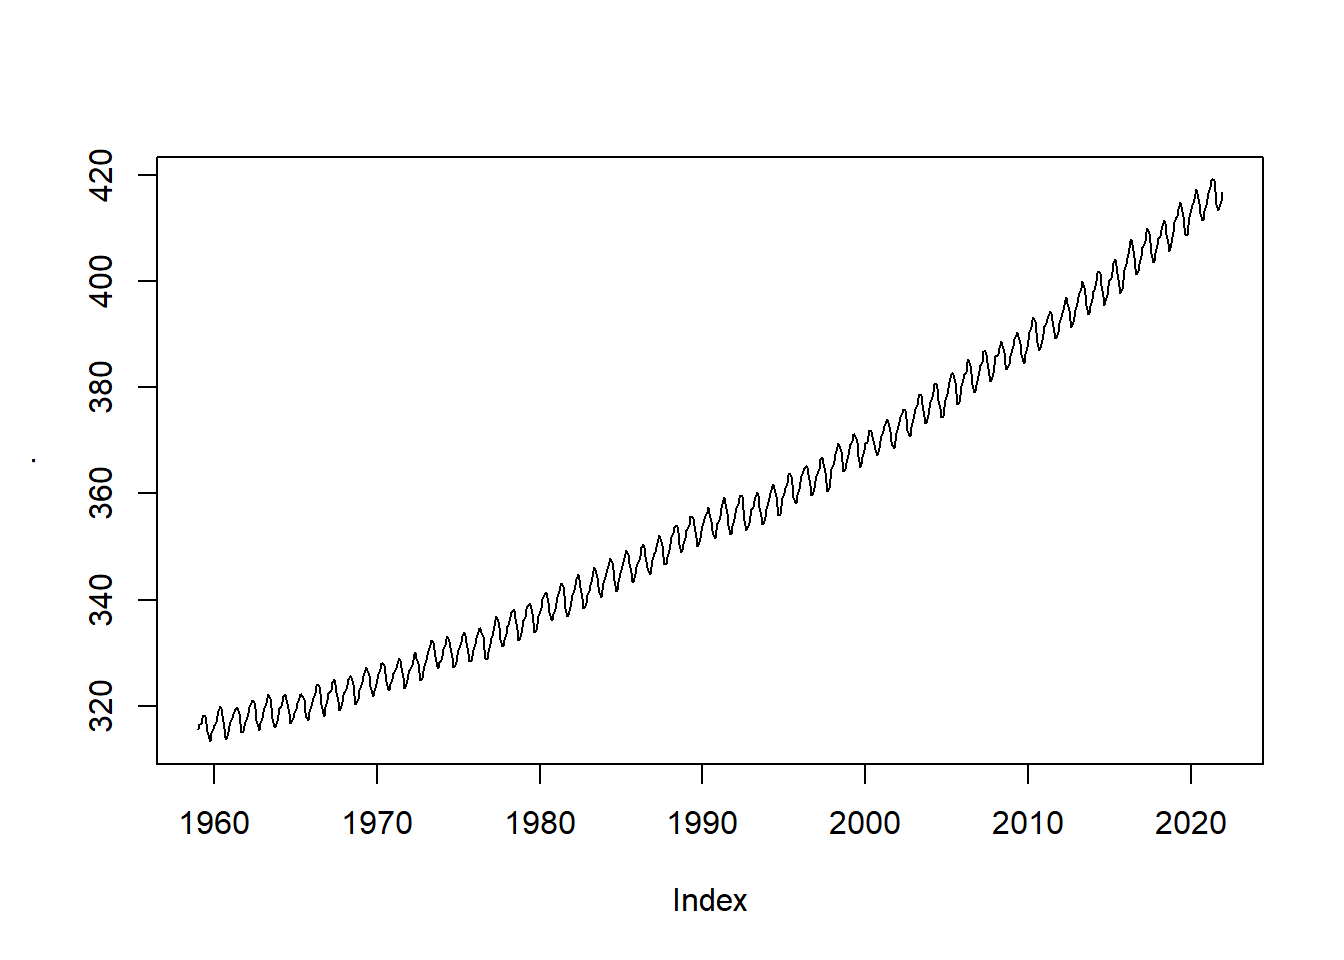
\includegraphics{_main_files/figure-latex/unnamed-chunk-4-1} \end{center}

\hypertarget{calculating-a-rolling-window}{%
\subsection{Calculating a Rolling Window}\label{calculating-a-rolling-window}}

\begin{Shaded}
\begin{Highlighting}[]
\NormalTok{dl\_dplyr\_rolling }\OtherTok{\textless{}{-}}\NormalTok{ dl\_dplyr }\SpecialCharTok{\%\textgreater{}\%}
  \FunctionTok{tq\_mutate}\NormalTok{(}
    \AttributeTok{select =}\NormalTok{ count,}
    \AttributeTok{mutate\_fun =}\NormalTok{ rollapplyr,}
    \AttributeTok{FUN =}\NormalTok{ mean,}
    \AttributeTok{width =} \DecValTok{7}\NormalTok{,}
    \AttributeTok{col\_rename =} \StringTok{"weekly\_avg"}
\NormalTok{  ) }\SpecialCharTok{\%\textgreater{}\%}
  \FunctionTok{tq\_mutate}\NormalTok{(}
    \AttributeTok{select =}\NormalTok{ count,}
    \AttributeTok{mutate\_fun =}\NormalTok{ rollapplyr,}
    \AttributeTok{FUN =}\NormalTok{ mean,}
    \AttributeTok{width =} \DecValTok{30}\NormalTok{,}
    \AttributeTok{col\_rename =} \StringTok{"monthly\_avg"}
\NormalTok{  )}

\NormalTok{weekly\_ts }\OtherTok{\textless{}{-}}\NormalTok{ dl\_dplyr\_rolling }\SpecialCharTok{\%\textgreater{}\%}
  \FunctionTok{select}\NormalTok{(date, weekly\_avg) }\SpecialCharTok{\%\textgreater{}\%}
  \FunctionTok{ts\_ts}\NormalTok{()}
\end{Highlighting}
\end{Shaded}

\begin{verbatim}
## [time]: 'date' [value]: 'weekly_avg'
\end{verbatim}

\begin{Shaded}
\begin{Highlighting}[]
\FunctionTok{ggplot}\NormalTok{() }\SpecialCharTok{+}
  \FunctionTok{geom\_line}\NormalTok{(}\AttributeTok{data =}\NormalTok{ dl\_dplyr, }\AttributeTok{mapping =} \FunctionTok{aes}\NormalTok{(}\AttributeTok{x =}\NormalTok{ date, }\AttributeTok{y =}\NormalTok{ count), }\AttributeTok{color =} \StringTok{"grey50"}\NormalTok{) }\SpecialCharTok{+}
  \FunctionTok{geom\_line}\NormalTok{(}\AttributeTok{data =}\NormalTok{ dl\_dplyr\_rolling, }\AttributeTok{mapping =} \FunctionTok{aes}\NormalTok{(}\AttributeTok{x =}\NormalTok{ date, }\AttributeTok{y =}\NormalTok{ weekly\_avg), }\AttributeTok{color =} \StringTok{"red"}\NormalTok{)}
\end{Highlighting}
\end{Shaded}

\begin{verbatim}
## Warning: Removed 6 row(s) containing missing values (geom_path).
\end{verbatim}

\begin{center}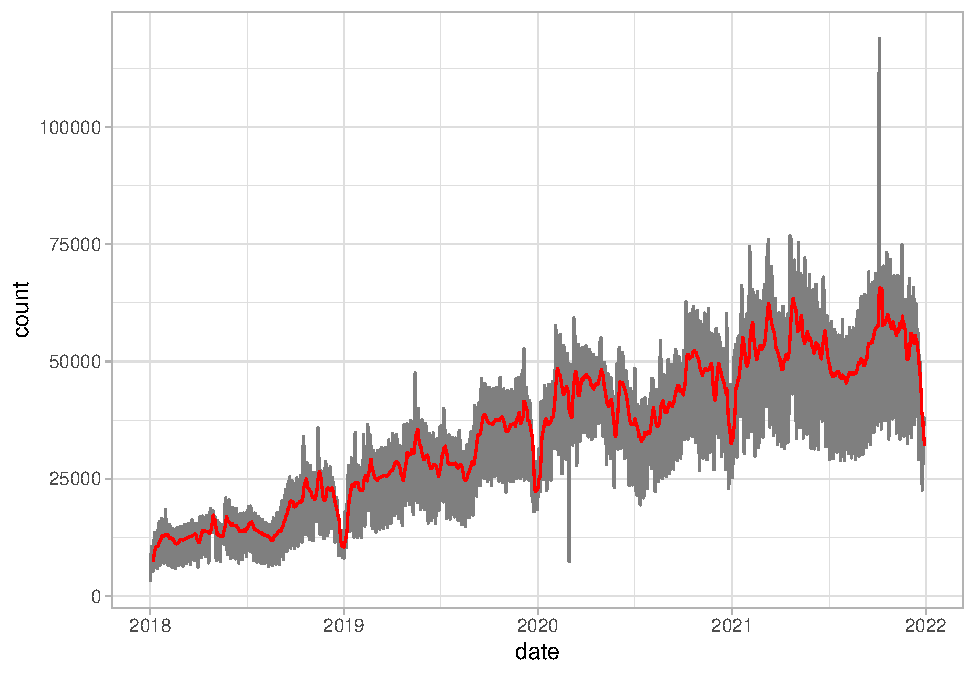
\includegraphics{_main_files/figure-latex/unnamed-chunk-6-1} \end{center}

\begin{Shaded}
\begin{Highlighting}[]
\NormalTok{dl\_rolling\_ts }\OtherTok{\textless{}{-}}\NormalTok{ dl\_dplyr\_rolling }\SpecialCharTok{\%\textgreater{}\%}
  \FunctionTok{select}\NormalTok{(}
\NormalTok{    date, weekly\_avg}
\NormalTok{  ) }\SpecialCharTok{\%\textgreater{}\%}
  \FunctionTok{ts\_ts}\NormalTok{()}
\end{Highlighting}
\end{Shaded}

\begin{verbatim}
## [time]: 'date' [value]: 'weekly_avg'
\end{verbatim}

\begin{Shaded}
\begin{Highlighting}[]
\NormalTok{dl\_rolling\_ts }\SpecialCharTok{\%\textgreater{}\%}
  \FunctionTok{decompose}\NormalTok{(}\AttributeTok{type =} \StringTok{"multiplicative"}\NormalTok{) }\SpecialCharTok{\%\textgreater{}\%}
  \FunctionTok{autoplot}\NormalTok{()}
\end{Highlighting}
\end{Shaded}

\begin{center}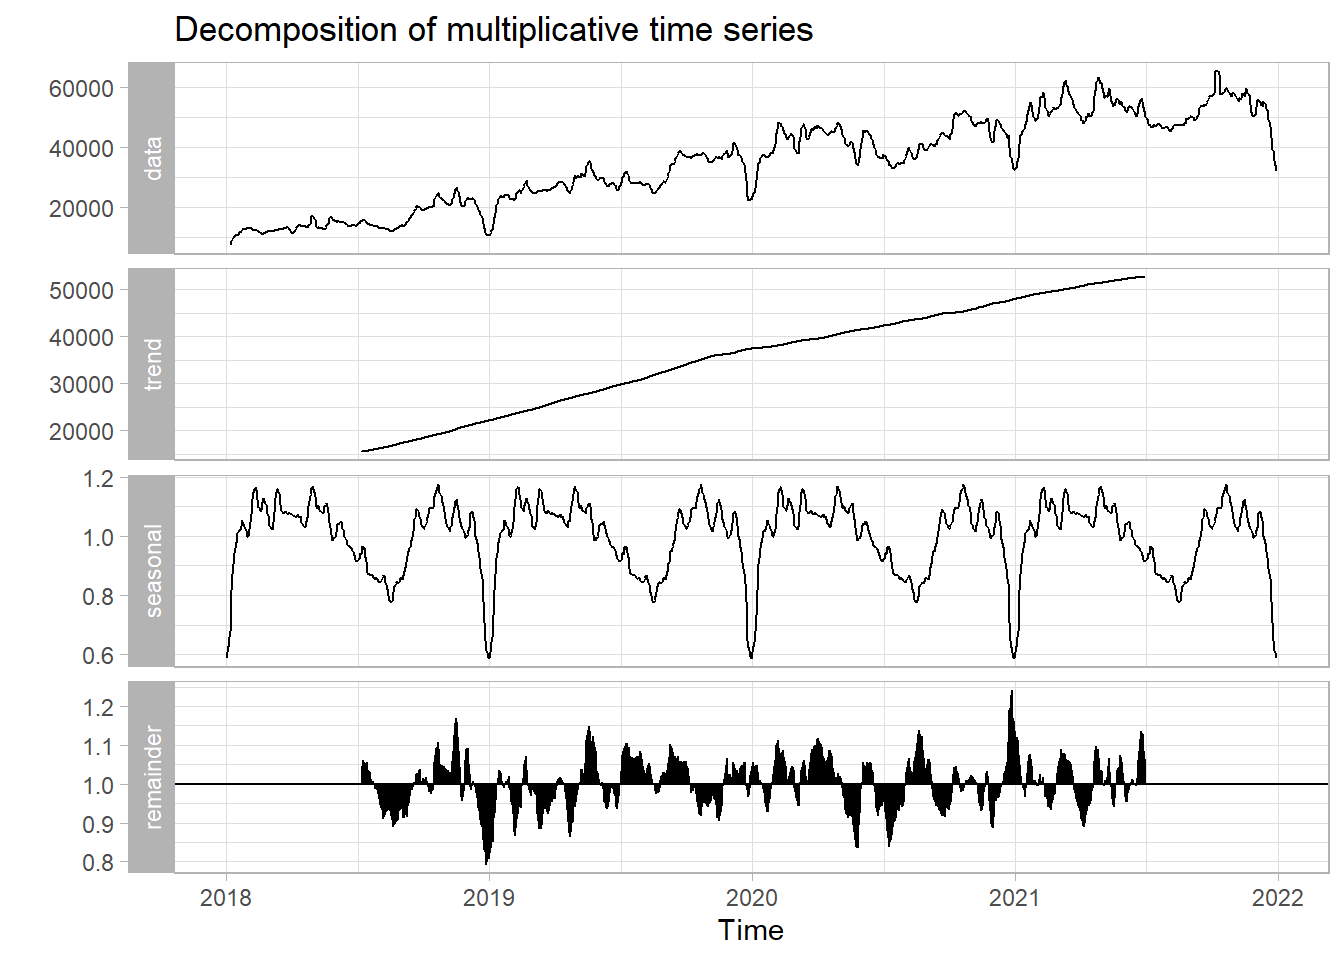
\includegraphics{_main_files/figure-latex/unnamed-chunk-7-1} \end{center}

\hypertarget{expanding-window}{%
\chapter{Expanding Window}\label{expanding-window}}

\begin{itemize}
\tightlist
\item
  Fixed lower bound
\item
  Moving upper bound
\end{itemize}

\begin{Shaded}
\begin{Highlighting}[]
\NormalTok{dl\_expand }\OtherTok{\textless{}{-}}\NormalTok{ dl\_dplyr }\SpecialCharTok{\%\textgreater{}\%} 
  \FunctionTok{mutate}\NormalTok{(}
    \AttributeTok{mean\_expand =} \FunctionTok{cummean}\NormalTok{(count),}
    \AttributeTok{cum\_sum =} \FunctionTok{cumsum}\NormalTok{(count)}
\NormalTok{  )}

\NormalTok{expand\_ts }\OtherTok{\textless{}{-}}\NormalTok{ dl\_expand }\SpecialCharTok{\%\textgreater{}\%} 
  \FunctionTok{select}\NormalTok{(date, mean\_expand) }\SpecialCharTok{\%\textgreater{}\%} 
  \FunctionTok{ts\_ts}\NormalTok{()}
\end{Highlighting}
\end{Shaded}

\begin{verbatim}
## [time]: 'date' [value]: 'mean_expand'
\end{verbatim}

\begin{Shaded}
\begin{Highlighting}[]
\FunctionTok{ggplot}\NormalTok{() }\SpecialCharTok{+}
  \FunctionTok{geom\_line}\NormalTok{(}\AttributeTok{data =}\NormalTok{ dl\_dplyr, }\FunctionTok{aes}\NormalTok{(}\AttributeTok{x =}\NormalTok{ date, }\AttributeTok{y =}\NormalTok{ count), }\AttributeTok{color =} \StringTok{"gray50"}\NormalTok{) }\SpecialCharTok{+}
  \FunctionTok{geom\_line}\NormalTok{(}\AttributeTok{data =}\NormalTok{ dl\_expand, }\FunctionTok{aes}\NormalTok{(}\AttributeTok{x =}\NormalTok{ date, }\AttributeTok{y =}\NormalTok{ mean\_expand), }\AttributeTok{color =} \StringTok{"red"}\NormalTok{) }\SpecialCharTok{+} 
  \FunctionTok{geom\_line}\NormalTok{(}\AttributeTok{data =}\NormalTok{ dl\_dplyr\_rolling, }\FunctionTok{aes}\NormalTok{(}\AttributeTok{x =}\NormalTok{ date, }\AttributeTok{y =}\NormalTok{ weekly\_avg), }\AttributeTok{color =} \StringTok{"blue"}\NormalTok{) }\SpecialCharTok{+} 
  \FunctionTok{geom\_line}\NormalTok{(}\AttributeTok{data =}\NormalTok{ dl\_dplyr\_rolling, }\FunctionTok{aes}\NormalTok{(}\AttributeTok{x =}\NormalTok{ date, }\AttributeTok{y =}\NormalTok{ monthly\_avg), }\AttributeTok{color =} \StringTok{"green"}\NormalTok{) }\SpecialCharTok{+} 
  \FunctionTok{theme\_light}\NormalTok{()}
\end{Highlighting}
\end{Shaded}

\begin{verbatim}
## Warning: Removed 6 row(s) containing missing values (geom_path).
\end{verbatim}

\begin{verbatim}
## Warning: Removed 29 row(s) containing missing values (geom_path).
\end{verbatim}

\begin{center}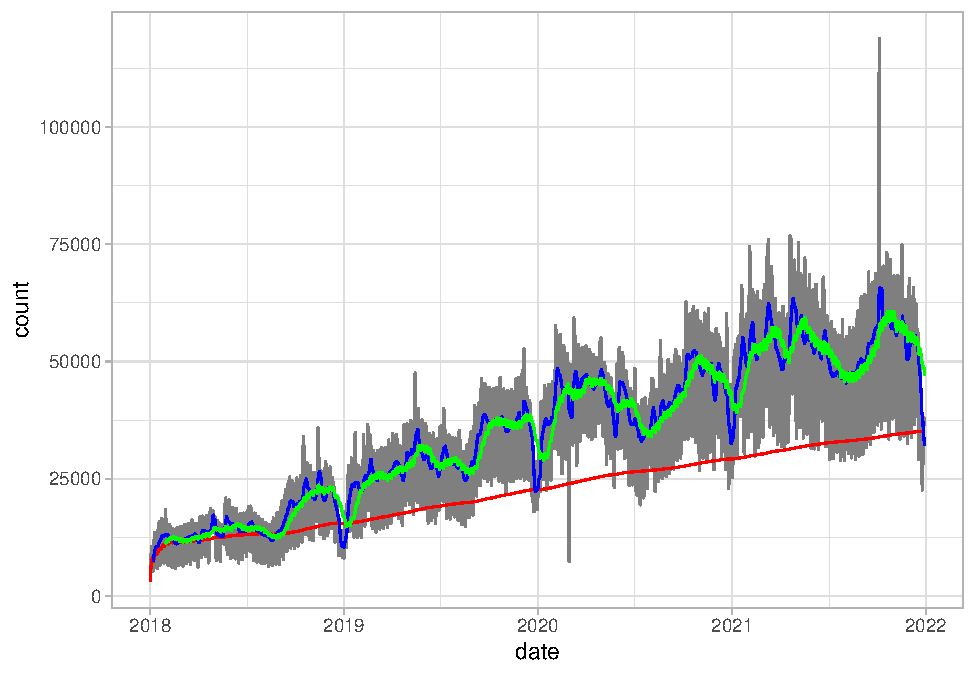
\includegraphics{_main_files/figure-latex/unnamed-chunk-9-1} \end{center}

\hypertarget{introduction-to-forecasting-in-r}{%
\chapter{Introduction to Forecasting in R}\label{introduction-to-forecasting-in-r}}

\hypertarget{methods-for-forecasting}{%
\section{Methods for Forecasting}\label{methods-for-forecasting}}

\hypertarget{exponential-smoothing}{%
\subsection{Exponential Smoothing}\label{exponential-smoothing}}

  \bibliography{book.bib,packages.bib}

\end{document}
